\subsubsection{Request a Taxi}
			To accompany this diagram, read the Scenario \hyperref[sec:TaxiRequiringScenario]{S.9}.

				\begin{table}[htpb]
					\centering
					\label{tab:TaxiRequestTable}
					\begin{tabularx}{\textwidth}{lp{9cm}}
						\hline
						\hline
							\textbf{Subject}
						& 
							\textbf{Description}\\
						\hline
							Actors	       &  Customer, myTaxiService Mobile Application, myTaxiService Server\\
						\hline
							Preconditions  &  Customer must be logged in, Customer must be on his homepage (see \hyperref[chome_m]{Customer Homepage}).\\
						\hline
							Execution      &  2.~Customer taps on the "Request Taxi" button.\\
										   &  3.~myTaxiService Mobile Application sends the requests to the Server.\\
										   &  4.~Customer waits for the acceptance.\\
										   &  5.~myTaxiService Mobile Application shows the acceptance notification.\\
										   &  6.~Customer waits for the Taxi.\\
						\hline
							Postconditions &  The Customer has request a taxi successfully.\\
						\hline
							Exceptions     &  1.~The Customer's GPS is off.\\
									
						\hline
						\hline
					\end{tabularx}
				\end{table}
				
				\begin{figure}[H]
					\centering
					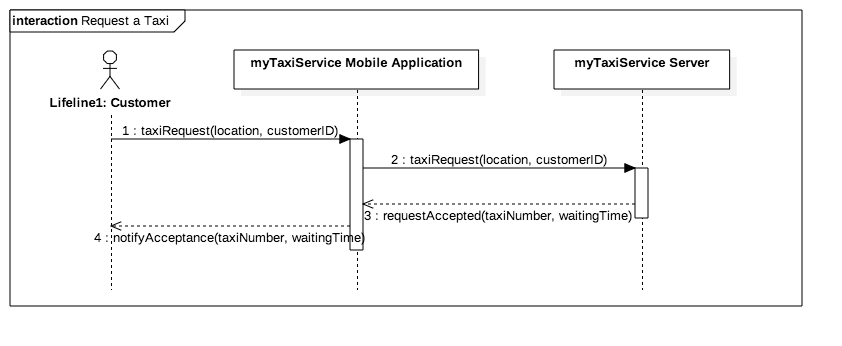
\includegraphics[width=\textwidth, scale=0.5]{IMG/InteractionDiagrams/TaxiRequest.png}
					\caption{Taxi Request Interaction Diagram}\label{sec:FigureTaxiRequest}
				\end{figure}